%% ------------------------------------------------------------------------- %%
\chapter{Problema}
\label{cap:problema}

Conforme o capítulo~\ref{cap:trabalhos-relacionados}, há várias pesquisas sobre o problema de perguntas e respostas no processamento de linguagem natural. Porém, como observado pelo trabalho da \cite{yao-2018} e apontado na seção~\ref{sec:algumas_referencias}, não há muita pesquisa sobre o problema de pares de perguntas e códigos-fontes. A partir de 2014, o StackOverFlow passou a disponibilizar a base de dados livremente. Diversas pesquisas foram feitas utilizando esta base de dados. E uma frente explorada pela \cite{yao-2018} e outros pesquisadores, é tentar resolver o problema de pergunta e resposta utilizando os dados do \textit{StackOverFlow}.

%------------------------------------------------------
\section{Problema de pares de perguntas e códigos-fontes do \textit{StackOverFlow}}

O problema de pares de perguntas e códigos-fontes já foi discutido na seção~\ref{sec:algumas_referencias}. E um dos obstáculos mencionados, é a obtenção de dados para o treinamento de modelos supervisionados. Desde 2014, o site \textit{StackOverFlow} disponibiliza sua base de perguntas e respostas através do site \cite{sof-2019}. Estes dados também podem ser consultados através do site \textit{BigQuery} do \cite{bigquery-2019} também. Numa consulta rápida, até 20 de março de 2019, havia mais de 17 milhões de perguntas em diversos tópicos de programação. Dúvidas sobre Python e SQL totalizam juntas mais de 2 milhões e meio.

\begin{figure}[h]
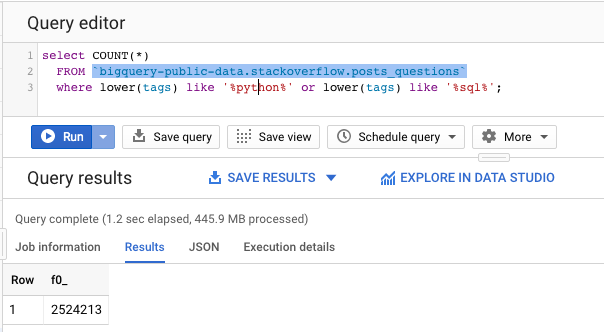
\includegraphics[width=12cm]{src/figuras/cap-problema/post-questions-python-sql-total.png}
\caption{Total de perguntas sobre Python e SQL no \textit{StackOverFlow} até 20 de março de 2019. Google and the Google logo are registered trademarks of Google LLC, used with permission.}
\label{fig:bigquery-total-questions-python-sql-stackoverflow}
\end{figure}

Somente com estes números, vê-se o potencial do \textit{StackOverFlow} como fonte de perguntas em linguagem natural e a sua solução em código fonte \cite{yao-2018}. Mas antes de utilizá-lo como fonte, é necessário levar em consideração quais assuntos é permitido fazer a pergunta. De acordo com o guia de boas práticas do \cite{stackoverflow-questions-topics-2019}, são permitidas perguntas sobre:

\begin{itemize}
    \item um problema específico de programação
    \item um algoritmo de programação
    \item ferramentas de programação
    \item problemas referentes a desenvolvimento de software
\end{itemize}

Analisando estes tipos de perguntas, uma pergunta sobre ferramentas de programação, dificilmente levará a uma resposta cuja solução seja um trecho de código-fonte. E se analisar cada um dos tópicos, verifica-se que nem todas as dúvidas vão levar a uma resposta com trechos de código-fonte. Muitas vezes, a resposta é somente uma orientação.

Levando isso em consideração, \citeauthor{yao-2018} coletou a partir da base aberta de questões e respostas do \cite{stackoverflow-questions-topics-2019}, somente perguntas do tipo \textit{how-to-do-it} referentes as linguagens \textit{SQL} e \textit{Python}. Perguntas do tipo \textit{how-to-do-it}, normalmente tem apenas uma resposta curta e direta cuja solução é um trecho de código-fonte. 

Ao final, foi coletado aproximadamente 148 mil pares de perguntas e trechos de código-fonte em \emph{Python} e em torno de 120 mil em \emph{SQL}. Os trechos de códigos-fontes foram extraídas das respostas aceitas\footnote{Resposta aceita contém um sinal de verificação verde. Esta resposta deve ser marcada como aceita pelo usuário que fez a pergunta.} pelos usuários\footnote{Usuário refere-se ao usuário que fez a pergunta no \textit{StackOverFlow}}. Uma resposta aceita no \textit{StackOverFlow} pode conter múltiplos trechos de códigos-fontes. A tabela~\ref{table:exemplo-pergunta-stack-over-flow-how-to-do-it} tem um exemplo de uma pergunta no qual a resposta aceita pelo usuário contém múltiplos trechos de código-fonte.

Para \cite{yao-2018}, um trecho de código-fonte é solução quando o usuário consegue resolver o problema somente baseado nele.
De acordo com esta definição, do conjunto \emph{\{C1, C2, C3, C4\}} de trechos do exemplo da tabela~\ref{table:exemplo-pergunta-stack-over-flow-how-to-do-it}, somente os \emph{C1} e \emph{C3} são consideradas soluções. \emph{C2} não é solução pois somente apresenta um exemplo de uso da função. E \emph{C4} é apenas um lembrete adicional ao usuário.

Múltiplos trechos de código-fonte na resposta é comum segundo \cite{yao-2018}. Estes representam mais de 44\% das respostas coletadas em \textit{Python} e mais de 34\% em \textit{SQL}. O usuário ao aceitar uma resposta, ele aceita a resposta como um todo, com todos os trechos de código-fonte como solução para o seu problema. Não há nenhuma indicação explícita apontando qual dos múltiplos trechos de código-fonte serve como solução. 

Para ter uma base de dados mais confiável, no qual questões estejam pareados com trechos de código-fonte que sejam soluções, \cite{yao-2018} empregou 4 estudantes de graduação com conhecimento em \textit{Python} e \textit{SQL} para marcar os trechos de código-fonte de uma resposta aceita. Para cada trecho de uma resposta aceita, o estudante deve marcar com a anotação \emph{1}, se ele acha que somente este trecho soluciona o problema. Caso contrário, ele anota com \emph{0}. Um trecho de código-fonte é considerado solução, caso dois estudantes anotem com \emph{1}.

Ao final, \cite{yao-2018} disponibilizou um conjunto contendo mais de 4800 pares de questões e trechos de códigos-fontes em \textit{Python} e mais de 3600 em \textit{SQL}. A partir destes dados, \cite{yao-2018} treinou um modelo de redes neurais recorrentes para responder a seguinte pergunta:

\emph{Dado um conjunto de trechos de código-fonte de uma resposta aceita no StackOverFlow. Qual destes trechos soluciona a questão em si?}

Este é um típico problema de pergunta e resposta, conforme mencionado na seção~\ref{sec:fundamentos}. 

Para ter uma base de dados confiável com maior precisão e \textit{recall}, \cite{yao-2018} propôs a seguinte tarefa:

\emph{Dado uma questão no \textit{StackOverFlow} e uma resposta aceita com múltiplos trechos de código-fonte, qual dos trechos de código-fonte são soluções?}






\begin{table}[h!]
\centering
\begin{tabular}{ |p{14cm}| } 
 \hline
\textbf{Pergunta:} Elegant Python function to
convert CamelCase to snake\_case \\ \hline
\textbf{S1}: This is pretty thorough:

\begin{lstlisting}[language=python, caption={C1}]
 def convert(name):
   s1 = re.sub('(.)([A-Z][a-z]+)', r'\1_\2',name)
   return re.sub('([a-z0-9])([A-Z])',r'\1_\2',s1).lower()
\end{lstlisting}

\textbf{S2}: Works with all these (and doesn't harm already-un-cameled versions):

\begin{lstlisting}[language=python, caption={C2}]
 >>> convert('CamelCase')
'camel_case'
>>> convert('CamelCamelCase')
'camel_camel_case'
\end{lstlisting}

\textbf{S3}: Or if you're going to call it a zillion times, you can pre-compile the regexes:

\begin{lstlisting}[language=python, caption={C3}]
first_cap_re = re.compile('(.)([A-Z][a-z]+)')
all_cap_re = re.compile('([a-z0-9])([A-Z])')
def convert(name):
   s1 = first_cap_re.sub(r'\1_\2', name)
   return all_cap_re.sub(r'\1_\2', s1).lower()
\end{lstlisting}

\textbf{S4}: Don't forget to import the regular expression module
\begin{lstlisting}[language=python, caption={C4}]
import re
\end{lstlisting}

 \\ 
 \hline
\end{tabular}
\caption{Exemplo de pergunta \textit{how-to-do-it} no \textit{StackOverFlow} com resposta aceita que contém mais de 1 (um) trecho de código-fonte como solução \cite{yao-2018}. Referência: \url{https://stackoverflow.com/questions/1175208/elegant-python-function-to-convert-camelcase-to-snake-case}}
\label{table:exemplo-pergunta-stack-over-flow-how-to-do-it}
\end{table}




\subsection{Detalhes do dataset}

 - Tamanho do dataset inicial
 - Dados sobre as perguntas, respostas (tamanho, quantidade de palavras etc.)

%------------------------------------------------------
\section{Arquitetura proposta} 

- Uso da rede LSTM/CNN 
       - Utilizando cosine similarity
       - Uso do word2vec para pergunta (linguagem natural) e outro para código (linguagem estruturada) - Verificar também se é viável usar o artigo Deep contextualized word representations ELMo representation (ao invés de word2vec) (According to the article: "We show that
these representations can be easily added to
existing models and significantly improve the
state of the art across six challenging NLP
problems, including question answering, textual entailment and sentiment analysis." )





